% !TEX program = xelatex

\documentclass{resume}
\usepackage{graphicx}
\usepackage{tabu}
\usepackage{multirow}
\usepackage{zh_CN-Adobefonts_external} % 
%\usepackage{zh_CN-Adobefonts_external} % Simplified Chinese Support using external fonts (./fonts/zh_CN-Adobe/)
%\usepackage{zh_CN-Adobefonts_internal} % Simplified Chinese Support using system fonts

\begin{document}
\pagenumbering{gobble} % suppress displaying page number

\Large{
  \begin{tabu}{ c l r }
   \multirow{5}{1in}{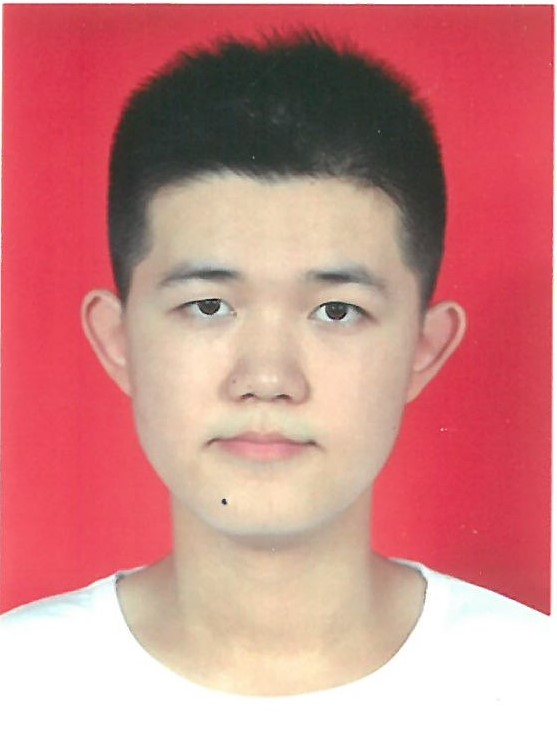
\includegraphics[width=0.88in]{avatar}} & \scshape{Ruan Yanhan} & \pbar{React}{0.8} \\
    & \email{ruanyanhan@whu.edu.cn} & \pbar{ES6}{0.8} \\
    & \phone{(+86) 173-1836-1969} & \pbar{Cesium}{0.5} \\
    & \linkedin[yo yo]{https://www.linkedin.com/in/yo-yo-974516289/} & \pbar{Express}{0.6} \\
    & \github[gitee.com/yohoyh]{https://gitee.com/yohoyh} & \pbar{Jquery}{0.6}
  \end{tabu}
}

\section{\faGraduationCap\ Education}
\datedsubsection{\textbf{Wuhan University (WHU)}, Wuhan, China}{2022 -- Present}
\textit{Master student} in Civil and Hydraulic engineering (Intelligence Research Direction), expected July 2024
\datedsubsection{\textbf{NORTHWEST A\&F UNIVERSITY (NWAFU)}, Shaanxi, China}{2018 -- 2022}
\textit{B.S.} in Water Resources and Hydropower Engineering

\section{\faUsers\ projects \& Experience}
\datedsubsection{\textbf{Carbon Neutralization Big Data Platform} Shanghai, China}{May. 2023 -- Present}
\role{collaborated with government departments}{React,Resium,ECharts,Antd,Express}
Brief introduction: The platform aims to enable carbon-neutral assessment and agricultural land information management on the islands.The main technical highlights are as follows:
\begin{itemize}
  \item Utilization of modern es6+ syntax: Leveraging the latest JavaScript syntax to improve development efficiency and code readability.
  \item Encapsulation of reusable utility functions: Implementation of function throttling for browser resize event, function debouncing for click event handling, and axios request/response interceptors. These utility functions enhance performance and code maintainability.
  \item Robust screen adaptation using vh, vw, rem,em: By employing units like vh, vw, rem, and em, the project ensures strong screen adaptability for various devices and screen sizes.
  \item Login validation through Higher Order Components (HOC): Incorporating HOCs to perform login validation and easily apply this functionality to components that require login validation, improving code reusability and maintainability.
  \item Enhanced performance and user experience with lazy loading: Implementing lazy loading to defer loading of components or resources, reducing unnecessary rendering and optimizing the performance and user experience of the application.
\end{itemize}

% Reference Test
%\datedsubsection{\textbf{Paper Title\cite{zaharia2012resilient}}}{May. 2015}
%An xxx optimized for xxx\cite{verma2015large}
%\begin{itemize}
%  \item main contribution
%\end{itemize}

% \section{\faCogs\ Skills}
% \begin{itemize}[parsep=0.5ex]
%   \item Programming Languages: C == Python > C++ > Java
%   \item Platform: Linux
%   \item Development: Web, xxx
% \end{itemize}

% \section{\faHeartO\ Honors and Awards}
% \datedline{\textit{\nth{1} Prize}, Award on xxx }{Jun. 2013}
% \datedline{Other awards}{2015}

\section{\faCalendarCheckO\ Awards}
\begin{itemize}[parsep=0.5ex]
  \item 2022 ZJU PAT - Professional Ability Test (95 / 100)
  \item 2022 ACM-ICPC excellence-award
  \item 2020 CMC second-prize
  \item 2020 MCM S-Award
  \item 2021 2 software works
\end{itemize}

\section{\faPlusCircle\ Miscellaneous}
\begin{itemize}[parsep=0.5ex]
  \item 114514
\end{itemize}

%% Reference
%\newpage
%\bibliographystyle{IEEETran}
%\bibliography{mycite}
\end{document}
